\graphicspath{{04-KL/Figures/}}

\section{KLOE-Light Calorimeter}
\label{Sect:KL}

\subsection{Introduction}
\label{SubSect:KL_Intro}
% v2 - Domizia Orestano reviewed this (Ludovico Tortora and Mariyan Bogomilov in cc)

The KLOE-Light (KL) pre-shower sampling calorimeter was composed of extruded lead foils in which scintillating fibres were placed. The volume ratio of scintillator to lead was approximately 2 to 1, ``lighter'' than the one of the KLOE experiment calorimeter~(1 to 1)~\cite{Ambrosino:2009zza}.

The fibres were 1\,mm diameter BICRON BCF-12, scintillating in the blue, spaced 1.35\,mm from each other within a layer. The distance between two layers was 0.98\,mm, one layer being shifted by half the fibre pitch with respect to the next.
Scintillation light was guided from each slab into a total of six PMTs (three on each side). Iron shields were fitted to each photomultiplier to
mitigate against large stray magnetic fields from the cooling channel. The signal from each PMT was sent to a shaping amplifier (SA) module, which shapes and stretches the signal in time in order to match the sampling rate of the flash ADCs (figure~\ref{fig:KL2} shows the design of a single slab).
A total of 7 slabs forms the whole detector, which has an active volume of 93\,cm$\times$93\,cm$\times$4\,cm.

With its 2.5 radiation lengths, the KL was used to distinguish muons from decay electrons providing energy deposition and timing information and to act as pre-shower in front of the EMR.
The detector has been used to estimate the level of pion contamination within the MICE muon beams to be around~1\%~\cite{2016JInst..11P3001A}.
\begin{figure}[htb!]
  \begin{center}
    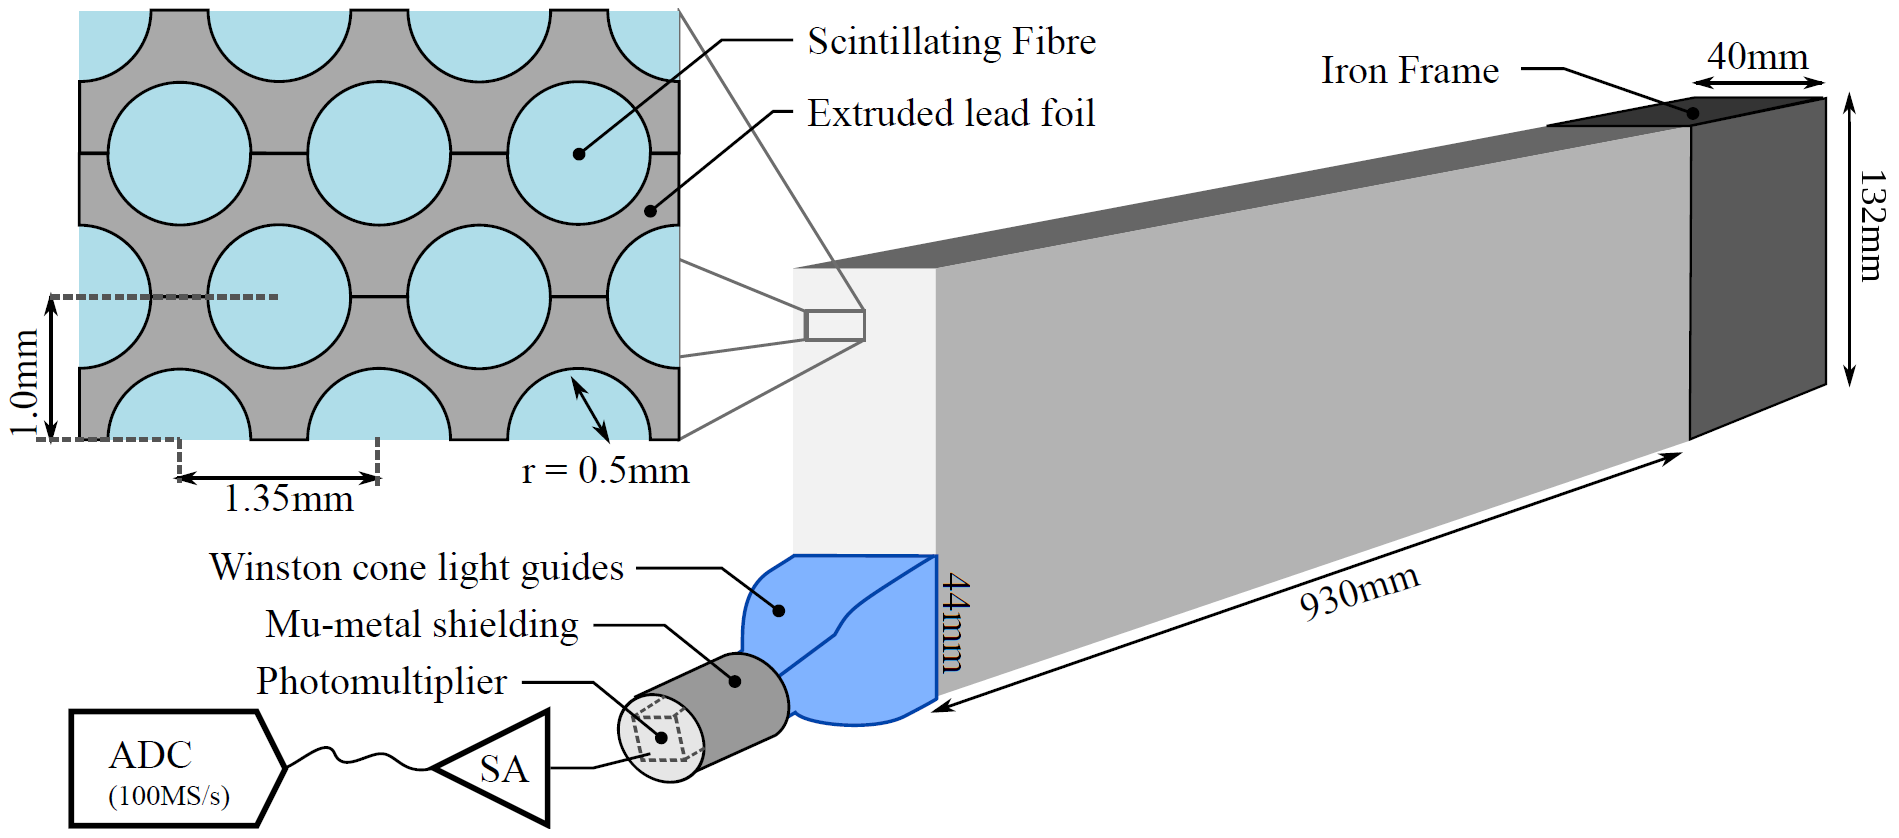
\includegraphics[width=0.8\columnwidth]{./04-KL/Figures/KL2.png}
    \caption{Single slab design of MICE KLOE-Light Calorimeter.}
    \label{fig:KL2}
  \end{center}
\end{figure}



\subsection{Performance}
\label{SubSect:KL_Performance}

The study of the KL response to different particle types (muons, pions and electrons) at different momenta was based on particle identification obtained by the time-of-flight detector, as shown in the example of~figure~\ref{fig:TOF_peaks}, by applying time cuts on the time-of-flight spectrum across the peaks of the different species. The performance is presented for beamline settings with nominal 140, 170, 200, 240 and 300\,MeV/$c$ momenta. The results presented below are obtained from the straight tracks runs (i.e. without magnetic fields in the trackers or focus coil). The KL response to muons, pions and electrons for all available momenta is presented in~figure~\ref{fig:KL3}. It is clear in the cases of muons and pions that they were below the minimum ionizing particle momenta since energy deposition decreases with momentum increasing. Actually the energy deposition is defined as the sum of ADC products from all cells in KL above a given threshold. The ADC product on the other hand is the product of the left and the right side of one slab divided by the sum of left and right side: $\text{ADC}_{\text{prod}} = 2 \times \text{ADC}_{\text{left}} \times \text{ADC}_{\text{right}} / (\text{ADC}_{\text{left}} + \text{ADC}_{\text{right}})$. The factor of 2 is present for normalisation. The product of two sides compensates the effect of attenuation.
  \begin{figure}[htb!]
	\begin{center}
  		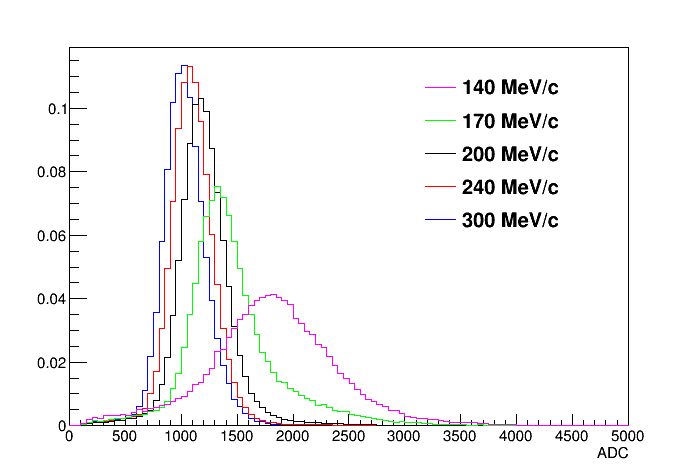
\includegraphics[width=0.49\columnwidth]{./04-KL/Figures/muon.png}
  		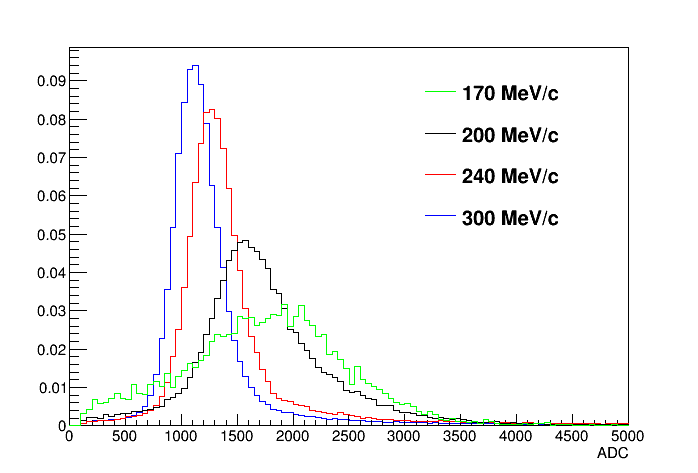
\includegraphics[width=0.49\columnwidth]{./04-KL/Figures/pion.png}
  		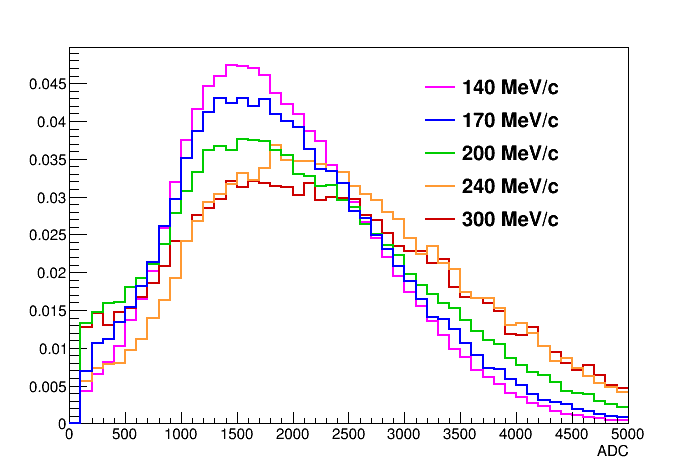
\includegraphics[width=0.49\columnwidth]{./04-KL/Figures/electron.png}
  		\caption{KL response to muons (top left), pions (top right) and electrons (bottom) for all available momenta. The charge deposited by particles in KL in arbitrary units is shown. All histograms are normalised to unity.}
  		\label{fig:KL3}
  	\end{center}
  \end{figure}
  
The comparison of energy deposition of muon, pions and electrons for a fixed momentum is presented in ~figure~\ref{fig:KL4}. 
For example 300 MeV/$c$~(figure~\ref{fig:KL4}, bottom) muons and pions have almost the same distribution, while moving to lower energies pions have a broader distribution, experiencing hadronic interactions and loosing more energy.
%In the case of 300 MeV/c (figure~\ref{fig:KL_mu_to_pi}), where muons and pions have almost the same distribution, the tail of pions is fatter than muon one.
%This is due to the fact that pions experience strong interaction as well.
This pion behaviour has been used to estimate its contamination in muon samples~\cite{2016JInst..11P3001A}. 

%The number of fired KL cells by a single muon, electron or pion is given in ~figure~\ref{fig:KL_mult} for 240 MeV/c beam. For muons we expect one, in some cases two and almost never more fired cells depending on track inclination. Pions and electrons create avalanches in KL and electron ones is much wider than the pion ones as visible of number of KL cell hits. The same figure shows number of events when if there is a reconstructed TOF track, but no signal in KL above the threshold. This can be used to calculate efficiency of KL for the three species as a function of momentum. The results are presented in ~Table~\ref{tab:KL_eff} and shows that efficiency for muon registration is close to 99$\%$.

\begin{figure}[htb!]
 	\begin{center}
		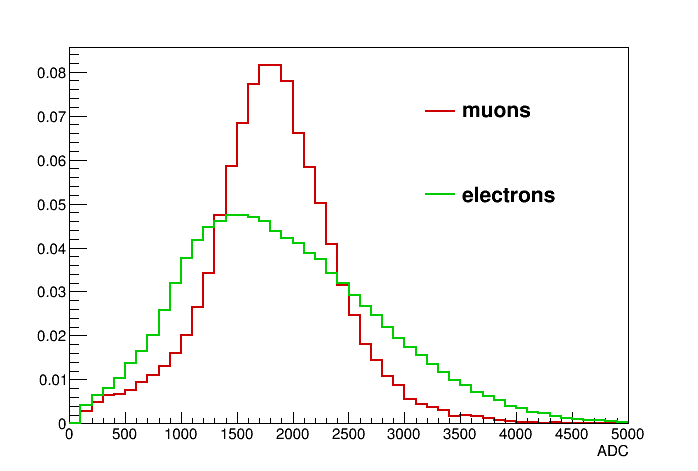
\includegraphics[width=0.45\columnwidth]{./04-KL/Figures/mu_vs_e_140MEV.png}
 		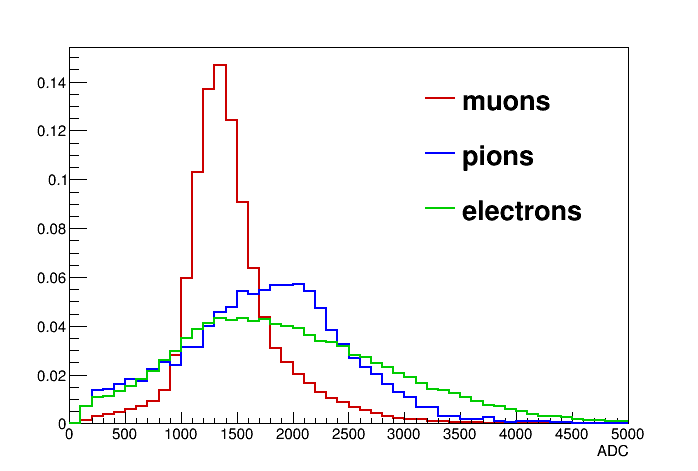
\includegraphics[width=0.45\columnwidth]{./04-KL/Figures/mu_vs_pi_vs_e_170MEV.png} 
 		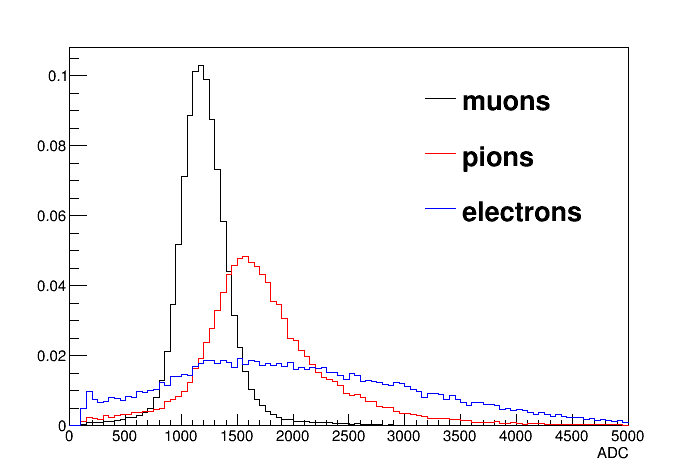
\includegraphics[width=0.45\columnwidth]{./04-KL/Figures/mu_vs_pi_vs_e_200MEV.png} 		
 		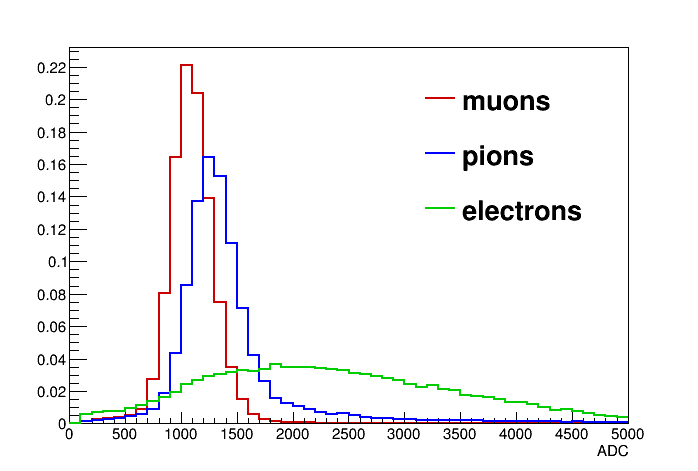
\includegraphics[width=0.45\columnwidth]{./04-KL/Figures/mu_vs_pi_vs_e_240MEV.png}  	
 		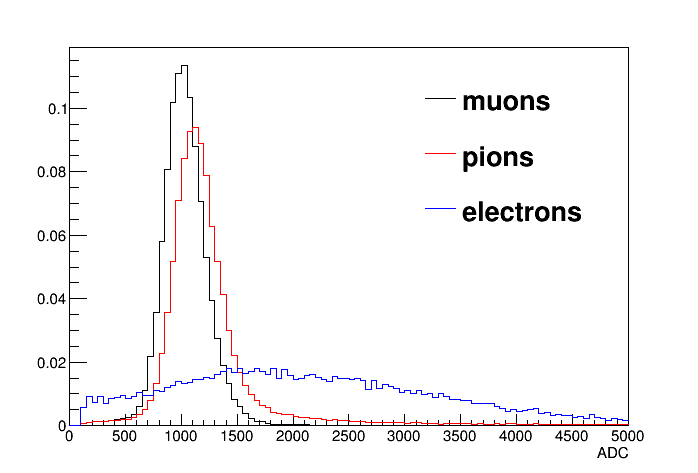
\includegraphics[width=0.45\columnwidth]{./04-KL/Figures/mu_vs_pi_vs_e_300MEV.png}
 		\caption{Comparison of energy deposition of muons, pions and electrons at 140 MeV/$c$ (top left), 170 MeV/$c$ (top right), 200 MeV/$c$ (middle left), 240 MeV/$c$ (middle right) and 300 MeV/$c$ (bottom).}
 		\label{fig:KL4}
 	\end{center}
\end{figure}

%\begin{figure}
%    	\begin{center}
%    		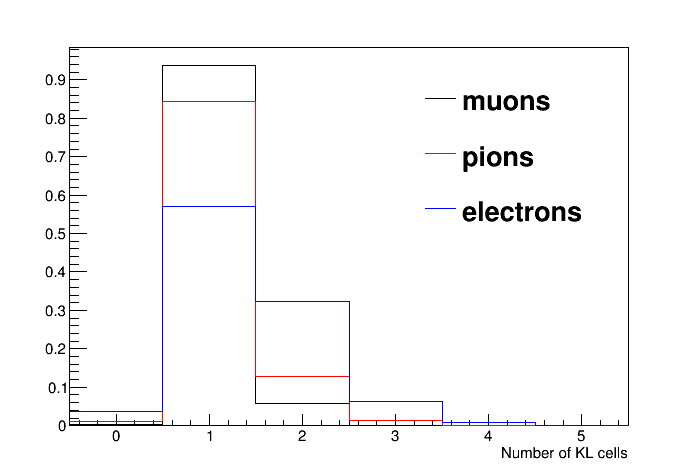
\includegraphics[width=0.4\columnwidth]{./04-KL/Figures/multiplicity_240MEV.png}  		
%    		\caption{Particle multiplicity for 240 MeV/c, i.e. number of KL cells fired.}
%    		\label{fig:KL_mult}
%    	\end{center}
%\end{figure}
       
  \begin{table}[!htb]
  	\begin{center}
  		\begin{tabular}{c|c|c|c|c|c} 
  			\textbf{Species} &\textbf{140 MeV/$c$} & \textbf{170 MeV/$c$} & \textbf{200 MeV/$c$}	&\textbf{240 MeV/$c$} &\textbf{300 MeV/$c$}\\
  			\hline
  			\textbf{electrons} & 0.95 $\pm$ 0.02  & 0.95 $\pm$ 0.01 & 0.94 $\pm$ 0.03 &  0.96 $\pm$ 0.02 &  0.95 $\pm$ 0.02 \\
  			\hline
  			\textbf{muons} &  0.97$\pm$ 0.02 & 0.99 $\pm$ 0.01  & 0.99 $\pm$  0.01 & 0.99 $\pm$ 0.01 & 0.99$\pm$ 0.01\\
  			\hline
  			\textbf{pions} &  n/a  & 0.89 $\pm$ 0.03  & 0.95 $\pm$ 0.03 & 0.97 $\pm$ 0.03 & 0.98$\pm$ 0.01\\
  		\end{tabular}
  		\caption{Efficiency of KL for electrons, muons and pions as a function of particle momentum. The conditions required the existence of a TOF track and signal in KL above the threshold. The uncertainties are statistical.}
  		\label{tab:KL_eff}
  	\end{center}
  \end{table}

In~figure~\ref{fig:KL_mc_vs_data} we show a simulation of KL response to 300 MeV/$c$ muons and pions and the distributions are compared with data.
The simulation takes into account the distribution of the photons in the scintillator fibres, the subsequent creation of photoelectrons on photomultiplier photocathodes and the response of the photomultipliers (where gain was around $2 \times 10^6$).
The agreement between data and simulation is very good.

%The simulation is done via following steps:
%\begin{itemize}
%	\item Smearing of produced photons in scintillator fibres. They obtain Poisson statistic so such is applied. In principal one can replace it with Gaussian because the number of photons created is  large enough for such an approximation.
%	\item Photoelectrons created on photomultiplier photocathode also have Poisson statistics. It cannot be replaced here with normal distribution because the number of photoelectrons is small enough so such an approximation is illegal.
%	\item Photomultiplier gain obtains also statistical properties but it is neither Poisson nor gauss. Nevertheless it turns out that for simplicity one can use Gaussian distribution with mean value equals to PMT gain and sigma of distribution equals to half of the gain. KL photomultipliers have gain $\sim 2 \times 10^6$, so their sigma was simply $10^6$.
%\end{itemize}

   \begin{figure}[htb!]
   	\begin{center}
   		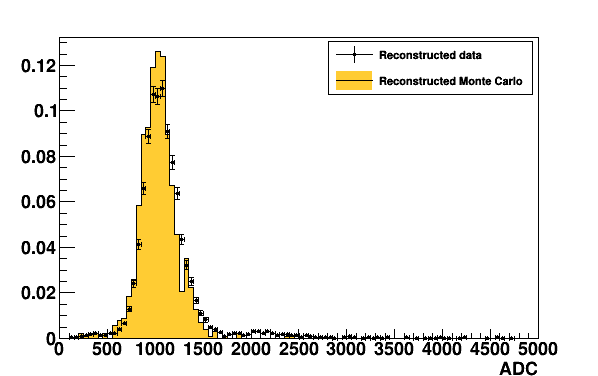
\includegraphics[width=0.4\columnwidth]{./04-KL/Figures/muon_mc_vs_data.png}  		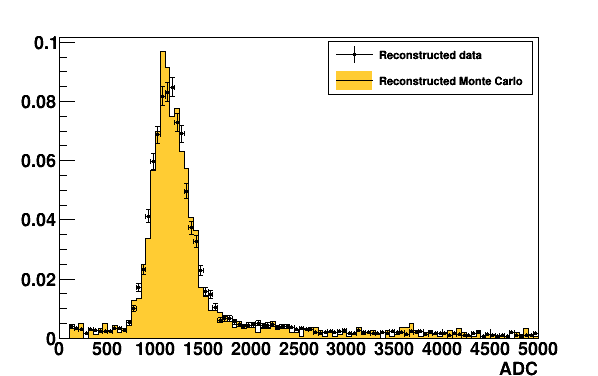
\includegraphics[width=0.4\columnwidth]{./04-KL/Figures/pion_mc_vs_data.png}
   		\caption{Comparison between data and Monte Carlo simulation of KL response to muons (left) and pions (right) at 300 MeV/$c$.}
   		\label{fig:KL_mc_vs_data}
   	\end{center}
   \end{figure}
